\chapter{Analysis Techniques}\label{ch:analysis}

This chapter provides some techniques to analyses FD schemes .

Techniques to analyse PDEs also exist, but the focus here is on the discrete schemes.

The analysis techniques will be especially explained from a practical side, rather than providing all the theory that they are based on. Obviously, references to work substantiating the claims made in this chapter will be provided. \todo{probably not necessary}

References to the origins of these techniques will be provided for the interested reader. 

\section{Matrices}
For several purposes, such as implementation in \texttt{MATLAB} and several analysis techniques described shortly, is useful to write a FD scheme in \textit{matrix form}. A matrix is a rectangular array with numerical elements and its dimensions are denoted using ``$row \times column$''. A $3\times 5$ matrix, for example, thus has $3$ rows and $5$ columns (see Figure \ref{fig:matrixA}). Along those lines, a \textit{row vector} is a matrix with $1$ row and more than $1$ column and a \textit{column vector} is a matrix with $1$ column and more than $1$ row. \SWcomment[If a matrix has only $1$ row and $1$ column, it can be used as a \textit{scalar}.] 

In this document, matrices and vectors are written using bold symbols. \SWcomment[Many notations exist, blabla $\bar a$ $\vec a$] A matrix is denoted by a capital letter -- such as $\A$ -- whereas vectors are decapitalised -- such as $\u$. An element in a matrix is denoted with a non-bold, decapitalised variable, where the subscripts indicate the indices of the row and column. For example, the element in the 2\textsuperscript{nd} row and the 4\th column of a matrix $\A$ is denoted as $a_{24}$.

A matrix or vector can be \textit{transposed}, and is indicated with the $T$ operator. Transposing a matrix $\A$ is denoted by $\A^T$.  means that the elements in the $i$\th row and the $j$\th column of the original matrix become the elements in the $j$\th row and the $i$\th column of the transposed matrix. Essentially the row and column indices of the elements inside the matrix get switched according to
\begin{equation}\label{eq:matrixTransposition}
    a_{ij} = a_{ji}.
\end{equation} 
Also see Figure \ref{fig:matrixTransp}. For a row vector, the transpose operation simply changes it to a column vector and vice versa. Another way of seeing a transpose is that all the elements get flipped over the \textit{main diagonal} of the matrix. The main diagonal comprises the elements $a_{ij}$ where $i=j$ and a transpose does not affect the location of these elements. 

\begin{figure}[h]
    \centering
    \subfloat[A $3\times 5$ matrix $\A$.\label{fig:matrixA}]{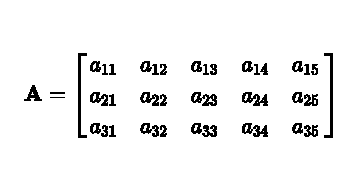
\includegraphics[width=0.45\textwidth]{figures/analysis/matrixA1.pdf}}\hspace{0.03cm}
    \subfloat[A transposed matrix $\A^T$ of size $5\times 3$.\label{fig:matrixAT}]{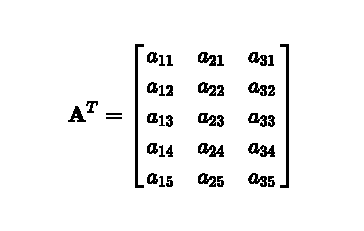
\includegraphics[width=0.45\textwidth]{figures/analysis/matrixAT1.pdf}}
    \caption{A matrix $\A$ and its transpose $\A^T$. The elements get flipped along the main diagonal of the matrix according to Eq. \eqref{eq:matrixTransposition}. \label{fig:matrixTransp}}
\end{figure}

\subsubsection{Matrix Multiplication}
In order for matrix multiplication (this includes matrix-vector multiplication) to be valid, the number of columns of the first matrix needs to be equal to the number of rows in the second matrix. The result will then be a matrix with a number of rows equal to that of the first matrix and a number of columns equal to that of the second matrix. See Figure \ref{fig:matrixVector} for reference.

As an example, consider the $L\times M$ matrix $
\A$ and a $M\times N$ matrix $\B$ with $L\neq N$. The multiplication $\A\B$ is defined as the number of columns of matrix $\A$ ($M$) is equal to the number of rows of matrix $\B$ (also $M$). The result, $\C$, is a $L \times N$ matrix. The multiplication $\B\A$ is undefined as the number of columns of the first matrix does not match the number of rows in the second matrix. A valid multiplication of two matrices written in their dimensions is
\begin{equation}
    \overbrace{(L\times M)}^{\A}\cdot \overbrace{(M\times N)}^{\B} = \overbrace{(L
    \times N)}^{\C}.
\end{equation}

A matrix can always be multiplied by a scalar (single number), which simply multiplies every element of the matrix by the scalar. 
\begin{figure}[h]
    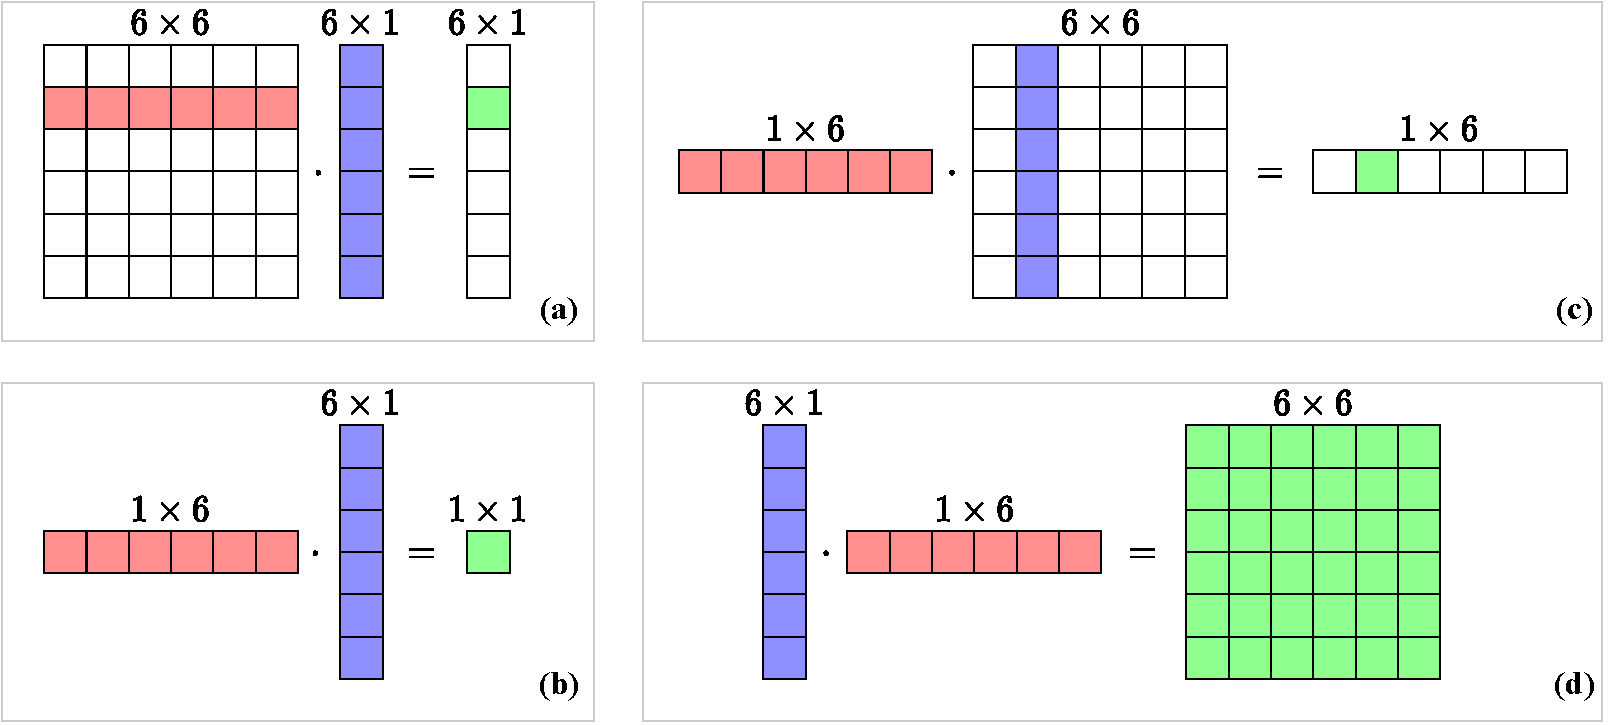
\includegraphics[width=\textwidth]{figures/analysis/matrixVector.pdf}
    \caption{Visualisation of valid matrix multiplications. The ``inner'' dimensions (columns of the left matrix and rows of the right) must match and result in a matrix with a size of ``outer'' dimensions (rows of the left matrix and columns of the right). \label{fig:matrixVector}}
\end{figure}

\subsection{In a FDTD context}
Matrix multiplication when working with FDTD methods usually involves multiplying a square matrix (with equal rows and columns) onto a column vector (see Figure \ref{fig:matrixVector}a). Consider a $(N+1)\times (N+1)$ square matrix $\A$ and a $(N+1) \times 1$ column vector $\u$. Multiplying these results in a $(N+1) \times 1$ column vector $\w$:
\begin{equation}
    \A\u = \w.
\end{equation}
Expanding this operation results in
\begin{equation}
    \underbrace{\begin{bmatrix}
        a_{00} & a_{01} & \hdots & a_{0N}\\
        a_{10} & a_{11} & \hdots & a_{2N}\\
        \vdots & \vdots & &\vdots\\
        a_{N0} & a_{N1} & \hdots & a_{NN}
    \end{bmatrix}}_{\A}
    \underbrace{\begin{bmatrix}
        u_0\\
        u_1\\
        \vdots\\
        u_N
    \end{bmatrix}}_{\u} = 
    \underbrace{\begin{bmatrix}
        a_{00}u_0 + a_{01}u_1 + \hdots + a_{0N}u_N\\
        a_{10}u_0 + a_{11}u_1 + \hdots + a_{1N}u_N\\
        \vdots\\
        a_{N0}u_0 + a_{N1}u_1 + \hdots + a_{NN}u_N
    \end{bmatrix}}_{\w}
\end{equation}
where the indexing starts at $0$ rather than $1$ here, as that relates better to a FDTD context.

\subsubsection{Operators in Matrix Form}
FD operators approximating spatial derivatives and averages can be written in matrix form and applied to a column vector $\u$ containing the state of the system at time index $n$. These matrices are square and their sizes depend on the number of grid points the system is described for and the boundary conditions. Not assuming a specific size for now, the FD operators in \eqref{eq:discFirstSpace} can be written in matrix form according to
% \setstackgap{L}{1.1\baselineskip}
% \fixTABwidth{T}
\setstackgap{L}{14pt}
\setstacktabbedgap{4pt}
\def\lrgap{\kern3pt}
\fixTABwidth{T}

\def\xbracketMatrixstack#1{\left[\lrgap\tabbedCenterstack{#1}\lrgap\right]}

\begin{equation*}
    \mathbf{D}_{x+} = \frac{1}{h}\xbracketMatrixstack{
        \ddots &\ddots & & & \mathbf{0}&\\
         & -1 & 1 & & & \\
        & & -1 & 1 & & \\
        & & & -1 & 1 & \\
        & & & & -1 & \ddots\\
        &\mathbf{0} & & & & \ddots
    }\qquad \mathbf{D}_{x-} = \frac{1}{h}\xbracketMatrixstack{
        \ddots & & & & \mathbf{0}&\\
        \ddots & 1 & & & & \\
        & -1 & 1 & & & \\
        & & -1 & 1 & & \\
        & & & -1 & 1 & \\
        &\mathbf{0} & & & \ddots & \ddots
    }
\end{equation*}

\begin{equation*}
    \mathbf{D}_{x\cdot} = \frac{1}{2h}\xbracketMatrixstack{
        \ddots &\ddots & & & \mathbf{0}&\\
        \ddots & 0 & 1 & & & \\
        & -1 & 0 & 1 & & \\
        & & -1 & 0 & 1 & \\
        & & & -1 & 0 & \ddots \\
        &\mathbf{0} & & & \ddots & \ddots
    }
\end{equation*}
% \begin{gather*}
%     \mathbf{D}_{x+} = \frac{1}{h}
%     \begin{bmatrix}
%         \ddots &\ddots & & & \mathbf{0}&\\
%          & -1 & 1 & & & \\
%         & & -1 & 1 & & \\
%         & & & -1 & 1 & \\
%         & & & & -1 & \ddots\\
%         &\mathbf{0} & & & & \ddots \\
%     \end{bmatrix}
%     \quad
%     \mathbf{D}_{x-} = \frac{1}{h}\begin{bmatrix}
%         \ddots & & & & \mathbf{0}&\\
%         \ddots & 1 & & & & \\
%         & -1 & 1 & & & \\
%         & & -1 & 1 & & \\
%         & & & -1 & 1 & \\
%         &\mathbf{0} & & & \ddots & \ddots \\
%     \end{bmatrix}\\
%     \\
%     \mathbf{D}_{x\cdot} = \frac{1}{2h}\begin{bmatrix}
%         \ddots &\ddots & & & \mathbf{0}&\\
%         \ddots & 0 & 1 & & & \\
%         & -1 & 0 & 1 & & \\
%         & & -1 & 0 & 1 & \\
%         & & & -1 & 0 & \ddots \\
%         &\mathbf{0} & & & \ddots & \ddots \\
%     \end{bmatrix}\\
% \end{gather*}
%
where the diagonal dots denote that the values on the respective diagonals continue until the top-left and bottom-right corners of the matrix. \todo{is this how you explain it?} The $\boldsymbol{0}$s indicate that the rest of the values in the matrix are zeros.

Averaging operators $\mxp$, $\mxm$ and $\mxd$ are defined in a similar way:

\begin{equation*}
    \mathbf{M}_{x+} = \frac{1}{2}\xbracketMatrixstack{
        \ddots &\ddots & & & \mathbf{0}&\\
         & 1 & 1 & & & \\
        & & 1 & 1 & & \\
        & & & 1 & 1 & \\
        & & & & 1 & \ddots\\
        &\mathbf{0} & & & & \ddots
    }
    \qquad
    \mathbf{M}_{x-} = \frac{1}{2}\xbracketMatrixstack{
        \ddots & & & & \mathbf{0}&\\
        \ddots & 1 & & & & \\
        & 1 & 1 & & & \\
        & & 1 & 1 & & \\
        & & & 1 & 1 & \\
        &\mathbf{0} & & & \ddots & \ddots
    }
\end{equation*}

\begin{equation*}    
    \mathbf{M}_{x\cdot} = \frac{1}{2}\xbracketMatrixstack{
        \ddots &\ddots & & & \mathbf{0}&\\
        \ddots & 0 & 1 & & & \\
        & 1 & 0 & 1 & & \\
        & & 1 & 0 & 1 & \\
        & & & 1 & 0 & \ddots \\
        &\mathbf{0} & & & \ddots & \ddots
    }
\end{equation*}

It is important to notice that only spatial operators are written in this matrix form and then applied to state vectors at different time steps ($\u^{n+1}$, $\u^n$ and $\u^{n-1}$). 

Finally, the identity matrix is a matrix with only $1$s on the diagonal and $0$s elsewhere as
\begin{equation*}
    \I = \xbracketMatrixstack{
        \ddots & & & & \mathbf{0}&\\
         & 1 & & & & \\
        & & 1 & & & \\
        & & & 1 & & \\
        & & & & 1 & \\
        &\mathbf{0} & & &  & \ddots
    }
\end{equation*}


\subsubsection{Schemes and Update Equations in Matrix Form}
With the spatial operators in matrix form presented above, the FD scheme of the 1D wave equation in \eqref{eq:1DwaveFDS} can be written in matrix form.

If the Dirichlet boundary conditions in \eqref{eq:discreteDirichlet} are used, the end points of the system do not have to be included in the calculation. The values of the grid function $\uln$ for $l\in \{1, \hdots, N-1\}$ can then be stored in a column vector according to $\u^n = [u_1^n, \hdots, u_{N-1}^n]^T$. Furthermore, $(N-1) \times (N-1)$ matrices $\mathbf{D}_{x+}$ and $\mathbf{D}_{x-}$ can be multiplied to get a same-sized matrix $\Dxx$:
\begin{equation}\label{eq:DxxDef}
    \Dxx = \mathbf{D}_{x+}\mathbf{D}_{x-} = \frac{1}{h^2}\xbracketMatrixstack{
        -2 & 1 & & &\mathbf{0}\\
        1 & -2 & 1 & & \\
        & \ddots & \ddots & \ddots & \\
        & & 1 & -2 & 1 \\
        \mathbf{0}& & & 1 & -2 
    }.
\end{equation}

If instead, Neumann boundary conditions in Eq. \eqref{eq:discreteDirichlet} are used, the values of $\uln$ for the full range $l\in \{0, \hdots, N\}$ need be stored as $\u^n=[u_0^n, \hdots, u_N^n]^T$ and the $(N+1) \times (N+1)$ matrix $\Dxx$ will be 
\begin{equation}
    \Dxx = \frac{1}{h^2}
    \xbracketMatrixstack{
        -2 & 2 & & &\mathbf{0}\\
        1 & -2 & 1 & & \\
        & \ddots & \ddots & \ddots & \\
        & & 1 & -2 & 1 \\
        \mathbf{0}& & & 2 & -2 
    },
\end{equation}
where the $2$s in the top and bottom row correspond to the multiplication by $2$ with $u_1^n$ and $u_{N-1}^n$ in Eqs. \eqref{eq:1DWaveLeftBound} and \eqref{eq:1DWaveRightBound} respectively.

Regardless of the boundary conditions, the FD scheme in \eqref{eq:1DwaveFDS} can be written in matrix form as
\begin{equation}\label{eq:1DwaveMatrix}
    \frac{1}{k^2}\left(\u^{n+1} - 2 \u + \u^{n-1}\right) = c^2 \Dxx \u^n,
\end{equation}
and rewritten to a matrix form of the update equation analogous to Eq. \eqref{eq:1DwaveUpdate}
\begin{equation}
    \u^{n+1} = (2\I + c^2k^2 \Dxx )\u^n - \u^{n-1}.
\end{equation}
The identity matrix is necessary here for correct matrix addition.

\subsection{Matrix Inverse}\label{sec:inverse}
If a matrix has the same number of rows as columns, it is called a \textit{square matrix}. Square matrices have special properties, one of which is that it (usually) can be \textit{inverted}. A square matrix $\A$ is invertable if there exists a matrix $\B$ such that
\begin{equation}
    \A \B = \B \A = \I. 
\end{equation}
This matrix $\B$ is then called the \textit{inverse} of $\A$ and can be written as $\A^{-1}$. Not all square matrices have an inverse. In this case, the matrix is called \textit{singular}. Rather than going through how to invert a matrix by hand, or determining whether it is singular, the following function in \texttt{MATLAB} will provide the inverse of a matrix \texttt{A}:
\begin{center}
    \texttt{A\_inverted = inv(A);}
\end{center}

The inverse of a \textit{diagonal matrix} (a matrix with non-zero elements on its main diagonal and the rest zeros) is obtained by replacing the diagonal elements by their reciprocal. So for a diagonal $3\times 3$ matrix, the following holds:
\begin{equation*}
    \xbracketMatrixstack{
        a_{11} & 0 & 0\\
        0 & a_{12} & 0\\
        0 & 0 & a_{33}
    }^{-1} =\quad 
    \xbracketMatrixstack{
        \frac{1}{a_{11}} & 0 & 0\\
        0 & \frac{1}{a_{12}} & 0\\
        0 & 0 & \frac{1}{a_{33}}
    }.
\end{equation*}

\subsection{Systems of Linear Equations}\label{sec:linearEquations}
Matrices can be conveniently used to solve \textit{systems of linear equations}, a set of linear equations containing the same set of variables. 

For example, take the system of linear equations
\begin{align*}
    x + z &= 6\\
    z - 3y &= 7\\
    2x + y + 3z &= 15
\end{align*}
with independent variables $x$, $y$ and $z$. The goal is to find a solution for these variables that satisfy all three equations. This system could be solved by hand using algebraic methods, but alternatively, the system can be written in matrix form:
\begin{equation}
    \A \u = \w.
\end{equation}
Here, column vector $\u$ contains the independent variables $x$, $y$, and $z$, matrix $\A$ contains the coefficients multiplied onto these variables and $\w$ contains the right-hand side, i.e., the coefficients not multiplied onto any of the variables:
\begin{equation*}
    \underbrace{\xbracketMatrixstack{
        1& 0& 1\\
        0& -3& 1\\
        2& 1& 3}}_{\A}
    \underbrace{\xbracketMatrixstack{
        x\\
        y\\
        z
    }}_{\u} = \underbrace{\xbracketMatrixstack{
        6\\
        7\\
        15
    }}_{\w}
\end{equation*}
We can then solve for $\u$ by taking the inverse of $\A$ (see Section \ref{sec:inverse}) and multiplying this onto $\w$
\begin{equation}
    \u = \A^{-1}\w.
\end{equation}
Generally, if X unknowns are described by X equations, the unknowns can be solved for using this method.

Solving a system of linear equations can be implemented in \texttt{MATLAB} by using the code given in Section \ref{sec:inverse} 
\begin{center}
    \texttt{u = inv(A) * w;}
\end{center}
or more compactly, by using the `\texttt{\textbackslash}' operator:
\begin{center}
    \texttt{u = A\textbackslash w;}
\end{center}

This method will come in handy in Section ...


\subsection{Eigenvalue Problems}\label{sec:eigenValueProblems}
A square matrix $\A$ is characterised by its \textit{eigenvalues} and corresponding \textit{eigenvectors}. In a FDTD context, these are usually associated with the modes of a system, where the eigenvalues relate to the modal frequencies and \todo{ask stefan} the eigenvectors to the modal shapes. Section \ref{sec:modalAnalysis} will provide more information on this.

To find these characteristic values for a $p\times p$ matrix $\A$, an equation of the following form must be solved 
\begin{equation}
    \A \boldPhi = \lambda \boldPhi.
\end{equation}
This is called is an \textit{eigenvalue problem} and has $p$ solutions (corresponding to the dimensions of $\A$). These are the $p$\th eigenvector $\boldPhi_p$ and the corresponding eigenvalue $\lambda_p$ which is calculated using
\begin{equation}
    \lambda_p = \eig_p(\A),
\end{equation}
where $\eig_p(\cdot)$ denotes the $p$\th eigenvalue of. Instead of delving too deep into eigenvalue problems and the process of how to solve them, an easy way to obtain the solutions using \texttt{MATLAB} is provided here:

\begin{center}\todo{Check code here!}
    \texttt{[phi, lambda] = eig(A, {\color[HTML]{A100F4}'vector'});}
\end{center}
The $p$\th eigenvector appears in the $p$\th column of $p\times p$ matrix \texttt{phi} and the eigenvalues are given in a $p \times 1$ column vector \texttt{lambda}. Note that the outcome is not sorted! To do this, do 
%
\todo{check whether this is necessary}
\begin{center}
    \begin{tabular}{l}
    \texttt{[lambda, order] = sort(lambda);}\\
    \texttt{phi = phi(:, order);}
    \end{tabular}
\end{center}

\section{Mathematical Tools and Product Identities}
Some useful mathematical tools used for the energy analysis techniques presented in Section \ref{sec:energyAnalysis} will be shown here.

\subsection{Inner products}
For two functions $f(x)$ and $g(x)$ defined for $x\in\D$ where $\mathcal{D} = [0,L]$, their $l_2$ inner product and $l_2$ norm are defined as
\begin{equation}\label{eq:contInnerProd}
    \langle f, g\rangle_\D = \int_\D fg dx \quad \text{and} \quad \lVert f \rVert_\D = \sqrt{\langle f, f \rangle_\D}.
\end{equation}
The discrete inner product of any (1D) grid function $f_l^n$ and $g_l^n$ defined for $l \in d$, with domain $d = \{0,\hdots,N\}$, is
\begin{equation}\label{eq:discInnerProd}
    \langle f^n, g^n \rangle_d = \sum_{l = 0}^N h f_l^n g_l^n,
\end{equation}
where the multiplication by $h$ is the discrete counterpart of $dx$ in the continuous definition in \eqref{eq:contInnerProd}. 

Also useful are the primed inner product
\begin{equation}\label{eq:primedInnerProd}
    \langle f^n, g^n \rangle_d' = \sum_{l=1}^{N-1} h f_l^n g_l^n + \frac{h}{2}f_0^ng_0^n + \frac{h}{2}f_N^ng_N^n,
\end{equation}
and the more general weighted inner product
\begin{equation}\label{eq:weightedInnerProd}
    \langle f^n, g^n \rangle_d^{\epsilon_\text{l}, \epsilon_\text{r}} = \sum_{l=1}^{N-1} h f_l^n g_l^n + \frac{\epsilon_\text{l}}{2}hf_0^ng_0^n + \frac{\epsilon_\text{r}}{2}hf_N^ng_N^n,
\end{equation}
which scale the boundary points of the regular inner product in \eqref{eq:discInnerProd}. 

\subsection{Summation by Parts}
Extremely useful when performing energy analysis on distributed systems is \textit{summation by parts}, which is the discrete counterpart to integration by parts. Although its application will be only be apparent when actually performing an energy analysis (see fx. Section \ref{sec:energyAnalysisString}) some definitions will be presented here for future reference.

Using the same functions $f(x)$ and $g(x)$ and domain $\D$ as before, and taking a spatial derivative of $g$, integration by parts is defined as
\begin{equation}
    \langle f, \px g \rangle_\D = -\langle \px f, g\rangle_\D + fg|_0^L
\end{equation}
where $fg|_0^L$ describes the boundary terms. One can observe that the spatial derivative is now applied to $f$ rather than $g$ and the sign of the inner product has inverted. 

Using discrete domain $d=\{0, \hdots, N\}$, summation by parts is defined as \cite{theBible}\todo{check whether this reference is necessary}
\begin{align}
    \langle f^n, \dxp g^n \rangle_d 
    %&= \sum_{l = 0}^N h f_l^n\frac{1}{h}\left(g_{l+1}^n - g_l^n\right)\nonumber\\
    % &= \sum_{l = 0}^N h\frac{1}{h}\left(f_l^n-f_{l-1}\right)g_l^n + f_N^ng_{N+1}^n - f_{-1}^ng_0^n \nonumber\\
    % &
    = -\langle \dxm f^n, g^n\rangle_d + f_N^ng_{N+1}^n - f_{-1}^ng_0^n\label{eq:summationByParts}
\end{align}
As one can observe, the 
It might be easier to see what happens with a derivation using $N = 2$ as an example. Suppressing the $n$ superscript for brevity, we get 
\begin{align*}
    \langle f, \dxp g \rangle_d &= \sum_{l = 0}^2 h f_l\frac{1}{h}\left(g_{l+1} - g_l\right),\\
    &= f_0g_1 - f_0g_0 + f_1g_2 - f_1g_1 + f_2g_3-f_2g_2,\\
    &= g_0(f_{-1}-f_0) - f_{-1}g_0 + g_1(f_0-f_1) + g_2(f_1-f_2) + f_2g_3,\\
    &= -g_0(f_0-f_{-1}) - g_1(f_1 - f_0) - g_2(f_2-f_1) + f_2g_3 - f_{-1}g_0,\\
    &= -\sum_{l=0}^2 h g_l\frac{1}{h}\left(f_l - f_{l-1}\right) + f_2g_3 - f_{-1}g_0,\\
    &= -\langle \dxm f, g\rangle_d + f_2g_3 - f_{-1}g_0.
\end{align*}
As $N=2$, the result is identical to Eq. \eqref{eq:summationByParts}

\subsection{Product identities}
Some useful identities used in this work are
\begin{subequations}
    \begin{align}
        (\dtd \uln)(\dtt \uln) &= \dtp \left(\frac{1}{2}(\dtm \uln)^2\right),\label{eq:prodIdentity1}\\
        (\dtd \uln)\uln &= \dtp \left(\frac{1}{2}\uln e_{t-}\uln\right),\label{eq:prodIdentity2}\\
        (\dtp \uln)(\mtp \uln) &= \dtp \left(\frac{1}{2}(\uln)^2\right),\label{eq:prodIdentity3}\\
        (\dtd \uln)(\mu_{t\cdot}\uln) &= \dtd\left(\frac{1}{2} (\uln)^2\right).\label{eq:prodIdentity4}
    \end{align}
\end{subequations}
Again, these can be used for spatial derivatives as well by substituting the `$t$' subscripts for `$x$'. Also to 

When an operator is applied to a product of two grid functions, the discrete counterpart of the product rule needs to be used according to
\begin{equation}
    \dtp (\uln\wln) = (\dtp \uln)(\mtp\wln) + (\mtp \uln)(\dtp \wln).
\end{equation}

\section{Frequency Domain Analysis}\label{sec:stabilityAnalysis}
Frequency domain analysis, also called Fourier analysis, is a way to determine various properties of a FD scheme, including conditions for stability. The process is similar to finding stability for digital filters. In essence, a FD scheme can be seen as a complex filter of which its coefficients are defined by physical parameters. \SWcomment[A mass-spring system finds a DSP equivalent in a resonator filter]

\subsubsection{Frequency domain representation and Ansatz}
FD schemes can be analysed by performing a \textit{z-transform}. The z-transform converts a discrete signal into a frequency domain representation, and is extensively used in the field of digital signal processing (DSP) to analyse the behaviour and especially stability of digital filters. To not go too much into detail here, the interested reader is referred to the very comprehensive explanation on the z-transform given in \cite[Ch. 5]{Park2010}. 

If a system is distributed in space, one can perform a spatial Fourier transform on a grid function. Frequency domain analysis in the distributed case is called von Neumann analysis which first appeared in \cite{Strikwerda1989} and is heavily used in \cite{theBible}. The discrete-time z-transform and discrete spatial Fourier transform performed on a 1D grid function are defined as \cite{theBible}
\begin{equation}
    \hat u  = \sum_{n=-\infty}^\infty \uln z^{-n}\qaq \tilde u = \sum_{l=-\infty}^\infty \uln e^{-jl\beta h}
\end{equation}
with complex number $z = e^{sk}$, complex frequency $s=j\omega + \sigma$ (more elaborated on in \ref{sec:modalAnalysis}) and real wavenumber $\beta$. Frequency domain analysis in 2D will be elaborated on in Section \ref{sec:analysis2D}.\todo{check if I should not refer to a subsection}

A shortcut to performing a full frequency domain analysis is to use a test solution, or \textit{ansatz}, and replace the grid functions by their transforms. The grid function for a 1D system can be replaced by an ansatz of the form (1D) \cite{Strikwerda1989}\todo{check reference}
\begin{equation}\label{eq:ansatz}
    u_l^n \ansatz z^n e^{jl\beta h}
\end{equation} 
where ``$\overset{\mathcal{A}}{\Longrightarrow}$'' indicates to replace the grid function with the ansatz (the shortcut to taking the full z-transform and spatial Fourier transform). 

Like in the DSP realm, the power of $z$ indicates a temporal shift, i.e., $z^{-1}$ is a one-sample delay. In a FDTD context, this corresponds to a time shift as seen in Section \ref{sec:FDoperators}. For spatially distributed systems, a shift in $l$ can be interpreted as a phase shift of a frequency with wavenumber $\beta$.\todo{check} See Table \ref{tab:zIdentities} for the frequency domain representation of of grid functions with their temporal and spatial indices shifted in different ways. 


{\renewcommand{\arraystretch}{1.2}

\begin{table}[h]
    \begin{center}
    \begin{tabular}{|c|c|c|}
        \hline
        Grid function & Ansatz & Result\\ \hline
        $u_l^n$ & $z^0 e^{j0\beta h}$ & $1$\\
        $u_l^{n+1}$ & $z^1 e^{j0\beta h}$ & $z$\\
        $u_l^{n-1}$ & $z^{-1} e^{j0\beta h}$ & $z^{-1}$\\
        $u_{l+1}^n$ & $z^0 e^{j1\beta h}$ & $e^{j\beta h}$\\
        $u_{l-1}^n$ & $z^0 e^{j(-1)\beta h}$ & $e^{-j\beta h}$\\
        $u_{l+2}^n$ & $z^0 e^{j2\beta h}$ & $e^{j2\beta h}$\\
        $u_{l-2}^n$ & $z^0 e^{j(-2)\beta h}$ & $e^{-j2\beta h}$\\
        $u_{l+1}^{n-1}$ & $z^{-1} e^{j1\beta h}$ & $z^{-1}e^{j\beta h}$\\
        $u_{l-1}^{n-1}$ & $z^{-1} e^{j(-1)\beta h}$ & $z^{-1}e^{-j\beta h}$\\\hline
    \end{tabular}
    \caption{Frequency-domain representation of a grid function using ansatz \eqref{eq:ansatz} with frequently appearing temporal and spatial shifts.\label{tab:zIdentities}}
    \end{center}
\end{table}
{\renewcommand{\arraystretch}{1}

%In the same way, using ``$\overset{\mathcal{Z}}{\Longrightarrow}$'' and ``$\overset{\mathcal{F}}{\Longrightarrow}$'' to denote a discrete z-transform and Fourier transform respectively,
Using these definitions, the effect of various operators on a grid function can be written in their frequency-domain representation. For systems distributed in space, the following trigonometric identities are extremely useful when performing the analyses \cite[p. 71]{Abramowitz1972}:
\begin{subequations}
    \begin{gather}
        \sin(x) = \frac{e^{jx} - e^{-jx}}{2j}\ \ \Rightarrow \ \ \sin^2(x) %= \frac{e^{j2x} - 2e^{jx-jx}+ e^{-j2x}}{-4} 
        = \frac{e^{j2x} + e^{-j2x}}{-4} + \frac{1}{2},\label{eq:sinIdentity}\\
        \cos(x) = \frac{e^{jx} + e^{-jx}}{2}\ \ \Rightarrow \ \ \cos^2(x) %= \frac{e^{j2x} + 2e^{jx-jx}+ e^{-j2x}}{4} 
        = \frac{e^{j2x} + e^{-j2x}}{4} + \frac{1}{2}.\label{eq:cosIdentity}
    \end{gather}
\end{subequations}
Take for example
\begin{equation*}
    \dxx \uln \ansatz \frac{1}{h^2}\left(e^{j\beta h} - 2 + e^{-j\beta h}\right).
\end{equation*}
Then, using $x = \beta h / 2$, identity \eqref{eq:sinIdentity} can be rewritten to 
\begin{equation*}
    e^{j\beta h} - 2 + e^{-j\beta h} = -4 \sin^2(\beta h / 2),
\end{equation*}
and substituted into the above to get
\begin{equation*}
    \dxx \uln \ansatz -\frac{4}{h^2}\sin^2(\beta h /2).
\end{equation*}
Examples of various temporal operators applied to grid functions in their frequency-domain representation are
\begin{equation}\label{eq:temporalAnsatz}
    \begin{aligned}
    \dtp \uln &\ansatz \frac{1}{k} \left(z - 1\right),& \dtm \uln &\ansatz \frac{1}{k} \left(1 - z^{-1}\right),\\
    \dtd \uln&\ansatz \dfrac{1}{2k} \left(z - z^{-1}\right), &\quad \dtt \uln&\ansatz\frac{1}{k^2} \left(z - 2 + z^{-1}\right)
    \end{aligned}
\end{equation}
and for spatial operators identity \eqref{eq:sinIdentity} can be used to obtain
\begin{subequations}
\begin{align}
    \dxx\uln&\ansatz \frac{-4}{h^2} \sin^2(\beta h / 2), \quad \label{eq:dxxAnsatz}\\
    \dxxxx \uln&\ansatz\frac{16}{h^4} \sin^4(\beta h / 2).\label{eq:dxxxxAnsatz}
\end{align}
\end{subequations}
Frequency domain analysis only works on linear and time-invariant (LTI) systems. Nonlinear\todo{FULL DOC SWEEP: nonlinear, non-linear or non linear} systems can be analysed using energy analysis (see Section \ref{sec:energyAnalysis}).\todo{not talking about nonlinear systems though}   

\subsubsection{Proving stability}
Just as with digital filters, the system is stable when the roots of the polynomial in $z$ are bounded by $1$ (unity)
\begin{equation}\label{eq:boundByUnity}
    |z| \leq 1.
\end{equation} 
In the FDTD context, the frequency-domain representation of a FD scheme results in a \textit{characteristic equation} -- usually a second-order polynomial- in $z$ and needs to satisfy condition \eqref{eq:boundByUnity} for all wave numbers $\beta$.
It can be shown that for a polynomial of the form 
\begin{equation}\label{eq:polynomialForm}
    z^2 + a^{(1)}z + a^{(2)}
\end{equation} 
its roots satisfy condition \eqref{eq:boundByUnity} when it abides the following condition \cite{theBible}
\begin{equation}\label{eq:condition214}
    |a^{(1)}| - 1 \leq a^{(2)} \leq 1.
\end{equation}
If $a^{(2)} = 1$, the simpler condition
\begin{equation}\label{eq:simplerCondition215}
    |a^{(1)}|\leq 2,
\end{equation}
suffices. 

\subsection{Mass-Spring System}
Recalling the FD scheme of the mass-spring system \eqref{eq:massSpringUpdate}
\begin{equation*}
    M \dtt \uln = -K \uln
\end{equation*} 
a frequency-domain representation can be obtained using the ansatz in \eqref{eq:ansatz} with $l = 0$. Using Table \ref{tab:zIdentities} and Eqs. \eqref{eq:temporalAnsatz} as a reference and substituting the definitions yields
\begin{equation*}
    \frac{M}{k^2}\left(z -2 +z^{-1}\right) = -K.
\end{equation*}
Gathering the terms and moving all to the left-hand side, the characteristic equation for the mass-spring system can be obtained:
\begin{equation}\label{eq:massSpringCharacteristic}
    z - \left(2-\frac{Kk^2}{M} \right) + z^{-1} = 0    
\end{equation}
To begin to prove stability, this equation needs to be written in the form found in \eqref{eq:polynomialForm}. Multiplying all the terms by $z$, and noticing that $a^{(2)} = 1$, we can continue with condition \eqref{eq:simplerCondition215}:
\begin{align*}
    \left|-2+\frac{Kk^2}{M}\right| &\leq 2,\\
    -2 \leq -2+\frac{Kk^2}{M} &\leq 2,\\
    0 \leq \frac{Kk^2}{M} &\leq 4.
\end{align*}
As $K$, $k$ and $M$ are positive variables, the first condition is always satisfied. The second condition is then easily solved for $k$ by
\begin{equation}\label{eq:stabilityMK}
    k \leq 2\sqrt{\frac{M}{K}}
\end{equation}
Recalling that $\omega_0 = \sqrt{K/M}$, Eq \eqref{eq:stabilityMK} can be more compactly written as 
\begin{equation}
    k \leq \frac{2}{\omega_0}.
\end{equation}\todo{Ask Stefan why he has $<$ and not $\leq$}

\subsection{1D Wave Equation}
This section will derive the stability condition for the 1D wave equation presented in Section \ref{sec:1DWave} using von Neumann analysis.

Recalling the FD scheme in \eqref{eq:1DwaveFDS},
\begin{equation*}
    \dtt \uln = c^2 \dxx \uln,
\end{equation*}
its frequency-domain representation can be obtained using the definitions in Eqs. \eqref{eq:temporalAnsatz} and \eqref{eq:dxxAnsatz}:
\begin{equation}
    \frac{1}{k^2}\left(z - 2 + z^{-1}\right) = -\frac{4c^2}{h^2}\sin^2\left(\beta h / 2)\right).
\end{equation}
Also recalling that
\begin{equation*}
    \lambda = \frac{ck}{h},
\end{equation*}
the characteristic equation of the 1D wave equation is
\begin{equation}\label{eq:1dWaveCharacteristic}
    z + \left(4\lambda^2\sin^2(\beta h / 2) -2\right) - z^{-1} = 0.
\end{equation}
% we can now perform von Neumann analysis. Moving all terms to the left-hand side and performing a z-transform and spatial Fourier transform we get:
% \begin{equation}\label{eq:zFDS}
%     z - 2(1-\lambda^2)1 - \lambda^2(e^{j\beta h}+e^{-j\beta h}) + z^{-1} = 0.
% \end{equation}
% Using the identity found in Eq. \eqref{eq:sinIdentity} with $\beta h = 2x \Rightarrow x = \beta h / 2$ we can rewrite \eqref{eq:zFDS} to:
% \begin{equation}
%      z - 2 + 2\lambda^2 +4\lambda^2(\sin^2({\beta h / 2}) - 1/2) - z^{-1} = 0,
% \end{equation}
% and rewriting this yields the characterstic equation shown in Eq. (6.38):
% \begin{equation}\label{eq:characteristic1D}
%      z + 2(2\lambda^2\sin^2(\beta h/2) - 1) + z^{-1} = 0.
% \end{equation}
% The roots are then given by (using $X = \lambda^2\sin^2(\beta h/2)$ for brevity):
% \begin{equation}
% \begin{aligned}\nonumber
%     z_\pm &= \frac{-2(2X-1) \pm \sqrt{4(2X-1)^2 - 4 \cdot 1 \cdot 1}}{2}\\
%     &= 1-2X \pm 1/2 \cdot \sqrt{4(2X-1)^2 - 4}\\
%     &= 1-2X \pm 1/2 \cdot \sqrt{4(4X^2-4X + 1) - 4}\\
%     &= 1-2X \pm 1/2 \cdot \sqrt{(4(4X^2 - 4X) + 4 - 4}\\
%     &= 1-2X \pm 1/2 \cdot \sqrt{4(4X^2 - 4X)}\\
%     &= 1-2X \pm 1/2 \cdot 2 \cdot \sqrt{4X^2 - 4X}\\
%     &= 1-2X \pm \sqrt{(1 - 2X)^2 - 1}\\
% \end{aligned}
% \end{equation}
% which results in the equation for the roots (right below (6.38) in section 6.2.2):
% \begin{equation}
%     z_\pm = 1-2\lambda^2\sin^2(\beta h/2) \pm \sqrt{(1 - 2\lambda^2\sin^2(\beta h/2))^2 - 1}.
% \end{equation}
The scheme is then stable if condition \eqref{eq:boundByUnity} is satisfied for the roots of \eqref{eq:1dWaveCharacteristic}. As the characteristic equation is of the form \eqref{eq:polynomialForm} with $a^{(2)} = 1$, stability is shown by abiding condition 
\eqref{eq:simplerCondition215} and when applied to the characteristic equation \eqref{eq:1dWaveCharacteristic} (after multiplication with $z$), it can be seen that
\begin{equation}\nonumber
    \begin{aligned}
        |4\lambda^2\sin^2(\beta h/2) - 2| &\leq 2,\\
        |2\lambda^2\sin^2(\beta h/2) - 1| &\leq 1,\\
        -1 \leq 2\lambda^2\sin^2(\beta h/2) - 1 &\leq 1,\\
        0 \leq 2\lambda^2\sin^2(\beta h/2)&\leq 2,\\
        0\leq \lambda^2\sin^2(\beta h/2) &\leq 1.
    \end{aligned}
\end{equation}
Observing that all terms in $\lambda^2\sin^2(\beta h/2)$ are squared, this term will always be non-negative and therefore always satisfy the first condition. Continuing with the second condition, and knowing that the $\sin^2(\beta h / 2)$-term is bounded by $1$ for all $\beta$, we arrive at the following stability condition:
\begin{equation*}
    \lambda \leq 1.
\end{equation*}
This is the CFL condition in \eqref{eq:CFL}. To obtain the stability condition in terms of the grid spacing, the definition for $\lambda$ is substituted and written in terms of the grid spacing
\begin{equation}
    h \geq ck,
\end{equation}
which is the stability condition given in Eq. \eqref{eq:1DWaveStabilityCond}.

\section{Energy Analysis}\label{sec:energyAnalysis}
Energy analysis techniques first appeared in (the first edition of) \cite{Gustafsson2013}\todo{shouldn't I just cite this one then?}

\SWcomment[(also see p. 54 in \cite{theBible}, specifically the section \textbf{Finite precision and round-off error for more references})]


For the 1D wave equation this means to multiply the scheme with $\left(\dtd \uln \right)$


The Hamiltonian or $\mathfrak{H}$


In implementation it can be very helpful to debug physical models...
One can plot the energy of the system and in a lossless system, the rate of change of the total energy should be 0, i.e.,
\begin{equation}\label{eq:unchangedEnergy}
    \delta_{t+}\mathfrak{h} = 0 \quad \Longrightarrow \quad \mathfrak{h}^n = \mathfrak{h}^0.
\end{equation}
.

Although the energy of a lossless system should be unchanged according to Eq. \eqref{eq:unchangedEnergy}, but in a finite precision simulation, ultra slight fluctuations of the energy should be visible due to rounding errors. 

Plotting energy should be within \textit{machine precision}, which mostly is in the range of $10^{-15}$

In this work, the focus of the energy analysis will be in discrete time...

The following steps can be followed to perform a full energy analysis of a FD scheme:
\subsubsection{Step 1: Obtain the rate of change of the energy (power) $\dtp \h$}
 The first step to energy analysis is to take the appropriate \textit{norm} of the scheme (see Eq. \eqref{eq:contInnerProd}). This yields the \textit{power} of the scheme, or in other words, the rate of change of the energy.

 \subsubsection{Step 2: Obtain the Energy $\h$ by isolating $\dtp$}
 As the interest lies in the energy, not the power, $\dtp$ must be isolated in the definition for the power.

\subsubsection{Step 3: Check Units}
To know that the previous steps have been carried out correctly, it is good to check whether the units of the resulting expression for $\h$ is indeed in Joules, or in SI units: kg $\cdot$ m$^2 \cdot $ s$^{-2}$. 

A first-order temporal difference operator will `add' one `s$^{-1}$'-unit (because of the $1/k$) and a first-order spatial difference operator will `add' one `m$^{-1}$'-unit ($1/h$). Along these lines, a second-order time or difference operator will `add' a `s$^{-2}$' ($1/k^2$) or `m$^{-2}$'-unit ($1/h^2$) respectively. It is important to note that the time shift operator ($e_{t-}$) does not influence the units. Finally, if the state $u$ describes a displacement in m, it will `add' this to the equation. If it describes anything else, it will `add' that.

\subsubsection{Step 4: Identify Kinetic Energy $\t$ and Potential Energy $\v$}
As a rule of thumb, the kinetic energy $\t$ contains `velocity squared' and the potential energy $\v$ is everything else. 

\subsubsection{Step 5: Implement the definitions for energy and debug the FD scheme}
In the end, the definition for $\h$ can be implemented and used as a check for whether the FD scheme has been implemented correctly.

\subsection{Mass-spring system}
\subsubsection{Step 1: Obtain $\dtp \h$}
The energy balance of the simple mass-spring system presented in Section \ref{sec:massSpringSystem} can be obtained by first taking the product of scheme \eqref{eq:massSpringFDS} with $(\dtd \un)$:
\begin{equation*}
    M(\dtd\un)(\dtt \un) = -K(\dtd\un)(\un)
\end{equation*}
Note that the inner product is not necessary as the system is not distributed. 

\subsubsection{Step 2: Isolate $\dtp$}
Identities \eqref{eq:prodIdentity1} and \eqref{eq:prodIdentity2}, can be used to get the following:
\begin{equation}
    \dtp \h = \dtp\left(\frac{M}{2}(\dtm\un)^2 + \frac{K}{2}\un e_{t-}\un\right) = 0,
\end{equation}
and the following energy balance results 
\begin{equation}\label{eq:energyBalanceMassSpring}
    \h = \frac{M}{2}(\dtm\un)^2 + \frac{K}{2}\un e_{t-}\un = 0,
\end{equation}

\subsubsection{Step 3: Check units}
As mentioned above, the energy $\h$ needs to be in Joules, or kg $\cdot$ m$^2 \cdot$ s$^{-2}$. Taking the terms in \eqref{eq:energyBalanceMassSpring} one-by-one and writing them in their units results in 
\begin{align*}
    \frac{M}{2}(\dtm\un)^2 &\overset{\text{in units}}{\xrightarrow{\hspace*{1cm}}} \quad\text{kg}\cdot(\text{s}^{-1}\cdot \text{m})^{2}= \text{kg}\cdot\text{m}^2\cdot\text{s}^{-2},\\
    \frac{K}{2}\un e_{t-}\un&\overset{\text{in units}}{\xrightarrow{\hspace*{1cm}}} \quad \text{N} \cdot \text{m}^{-1} \cdot \text{m}\cdot \text{m} = \text{kg}\cdot\text{m}^2\cdot\text{s}^{-2}.
\end{align*}
These have the correct units. 

\subsubsection{Step 4: Identifying $\t$ and $\v$}
As the first term in Eq. \eqref{eq:energyBalanceMassSpring} has a velocity-squared term in it, the following can be concluded:
\begin{equation}
    \t = \frac{M}{2}(\dtm\un)^2, \qaq \v = \frac{K}{2}\un e_{t-}\un.
\end{equation} 
\subsubsection{Step 5: Implementation}


\subsection{1D Wave Equation}
In order for the units in step 3

\subsubsection{Step 2: Isolate}

\subsection{Stability Analysis}
One can perform stability analysis using the energy analysis techniques presented here. To arrive at a condition the energy must be \textit{positive definite} 

As opposed to the frequency domain analysis presented in Section \ref{sec:stabilityAnalysis}, energy analysis techniques do not operate in the frequency domain. However, stability can be shown using the techniques presented here. Stability analysis using the energy method might even be considered more powerful than the frequency domain approach, as it also applies (to some degree) to non-linear and time-varying systems!

Rather than the roots of a characteristic equation needing to be bound by $1$, to arrive at a condition the energy must be \textit{positive definite}.


\SWcomment[1D wave stability from energy can be found in Section 6.2.7 in \cite{theBible}]

\section{Modal Analysis}
\label{sec:modalAnalysis}
Modes are the resonant frequencies of a system. The amount of modes that a discrete system contains depends on the amount of moving points. A mass-spring system thus has one resonating mode, but a FD scheme of the 1D wave equation with $N = 30$ and Dirichlet boundary conditions will have $29$ modes. This section will show how to analytically obtain the modes of an FD scheme implementing the 1D wave equation. 

We start by using the the matrix form of FD scheme \eqref{eq:1DwaveFDS} from Eq. \eqref{eq:1DwaveMatrix}
\begin{equation*}
    \frac{1}{k^2}\left(\u^{n+1}-2\u^n+\u^{n-1}\right) = c^2 \Dxx\u.
\end{equation*}
Following \cite{theBible} we assume a solution of the form $\u = z^n\boldPhi$ \todo{more explanation, perhaps refer to von neumann analysis in \ref{sec:stabilityAnalysis}}. Substituting this into the above equation yields the characteristic equation
\begin{equation}
    (z - 2 + z^{-1})\boldPhi = c^2k^2\Dxx \boldPhi.
\end{equation}
This is an eigenvalue problem (see Section \ref{sec:eigenValueProblems}) where the $p$\th solution $\boldPhi_p$ may be interpreted as the modal shape of mode $p$. The modal frequencies are the solutions to the following equations:
\begin{gather}
    z_p-2+z_p^{-1} = c^2k^2\text{eig}_p(\Dxx),\nonumber\\
    z_p+(-2-c^2k^2\text{eig}_p(\Dxx))+z_p^{-1}=0.
\end{gather}
\SWcomment[If the CFL condition for the scheme is satisfied, the roots will lie on the unit circle.] Furthermore, we can substitute a test solution $z_p=e^{j\omega_pk}$ with angular frequency of the $p$\th mode $\omega_p$ and solve for these:
\begin{align*}
    e^{j\omega_pk}+e^{-j\omega_pk}-2-c^2k^2\text{eig}_p(\Dxx)&=0,\\
    \frac{e^{j\omega_pk}+e^{-j\omega_pk}}{-4}+\frac{1}{2}+\frac{c^2k^2}{4}\text{eig}_p(\Dxx)&=0,
\end{align*}
and using Eq. \eqref{eq:sinIdentity} we get
\begin{align}
    \sin^2(\omega_pk/2)&+\frac{c^2k^2}{4}\text{eig}_p(\Dxx)=0,\nonumber\\
    \sin(\omega_pk/2)&=\frac{ck}{2}\sqrt{-\text{eig}_p(\Dxx)},\nonumber\\
    \omega_p &= \frac{2}{k}\sin^{-1}\left(\frac{ck}{2}\sqrt{-\text{eig}_p(\Dxx)}\right).
\end{align}

\subsection{One-Step Form}\label{sec:oneStepForm}
For more complicated systems, where the coefficients of $z$ and $z^{-1}$ in the characteristic equation are not identical for example, it is useful to rewrite the update in \textit{one-step form}. Although the eigenfrequency calculation needs to be done on a larger matrix, it allows for a more general and direct way to calculate the modal frequencies and damping coefficients per mode. 

If matrix $\A$ has an inverse, any scheme of the form
\begin{equation}\label{eq:modalForm}
    \A\u^{n+1}=\B\u^n + \C\u^{n-1},
\end{equation}
can be rewritten to
\begin{equation}\label{eq:oneStepForm}
    \underbrace{\begin{bmatrix}
        \u^{n+1}\\
        \u^n
    \end{bmatrix}}_{\w^{n+1}} = 
    \underbrace{\begin{bmatrix}
        \A^{-1}\B & \A^{-1}\C\\
        \I & \mathbf{0}
    \end{bmatrix}}_{\Q}
    \underbrace{\begin{bmatrix}
        \u^n\\
        \u^{n-1}
    \end{bmatrix}}_{\w^n}
\end{equation}
which relates the unknown state of the system to the known state through matrix $\Q$ which encompases the scheme. The sizes of the identity matrix $\I$ and zero matrix $\mathbf{0}$ are the same size as $\A, \B$ and $\C$.

Again we can assume solutions of the form $\w = z^n\boldPhi$ \SWcomment[(where $\boldPhi$ is less-trivially connected to the modal shapes)] and get
\begin{equation}
    z\boldPhi = \Q\boldPhi ,
\end{equation}
which can be solved for the $p$th eigenvalue as
\begin{equation}
    z_p = \text{eig}_p(\Q).
\end{equation}
As the scheme could exhibit damping, the test solution needs to include this and will be $z_p = e^{s_pk}$ with complex frequency $s_p= j\omega_p + \sigma_p$ and damping of the $p$th eigenfrequency $\sigma_p$. Substituting the test solution and solving for $s_p$ yields
\begin{align}
    e^{s_pk} &= \text{eig}_p(\Q),\nonumber\\
    s_p &= \frac{1}{k}\ln \left(\text{eig}_p(\Q)\right).\label{eq:sp}
\end{align}
Solutions for the frequency and damping for the $p$th eigenvalue can then be obtained through
\begin{equation}
    \omega_p = \mathfrak{I}(s_p) \quad \text{and} \quad \sigma_p = \mathfrak{R}(s_p),
\end{equation}
where $\mathfrak{I}(\cdot)$ and $\mathfrak{R}(\cdot)$ denote the ``imaginary part of'' and ``real part of'' respectively. 

As the elements of $\Q$ are real-valued, the solutions $s_p$ in Eq. \eqref{eq:sp} come in complex conjugates. For analysis, only the $\mathfrak{I}(s_p)\geq 0$ should be considered as these correspond to non-negative frequencies. 

\section{Dispersion analysis}\label{sec:dispersionAnalysis}
